\chapter{Resultados de los distintos modelos \gls{randomforest}}
\label{appendix:resultadosRF}

\section{Intervalo 0.2s}

\begin{figure}[H]
    \centering
    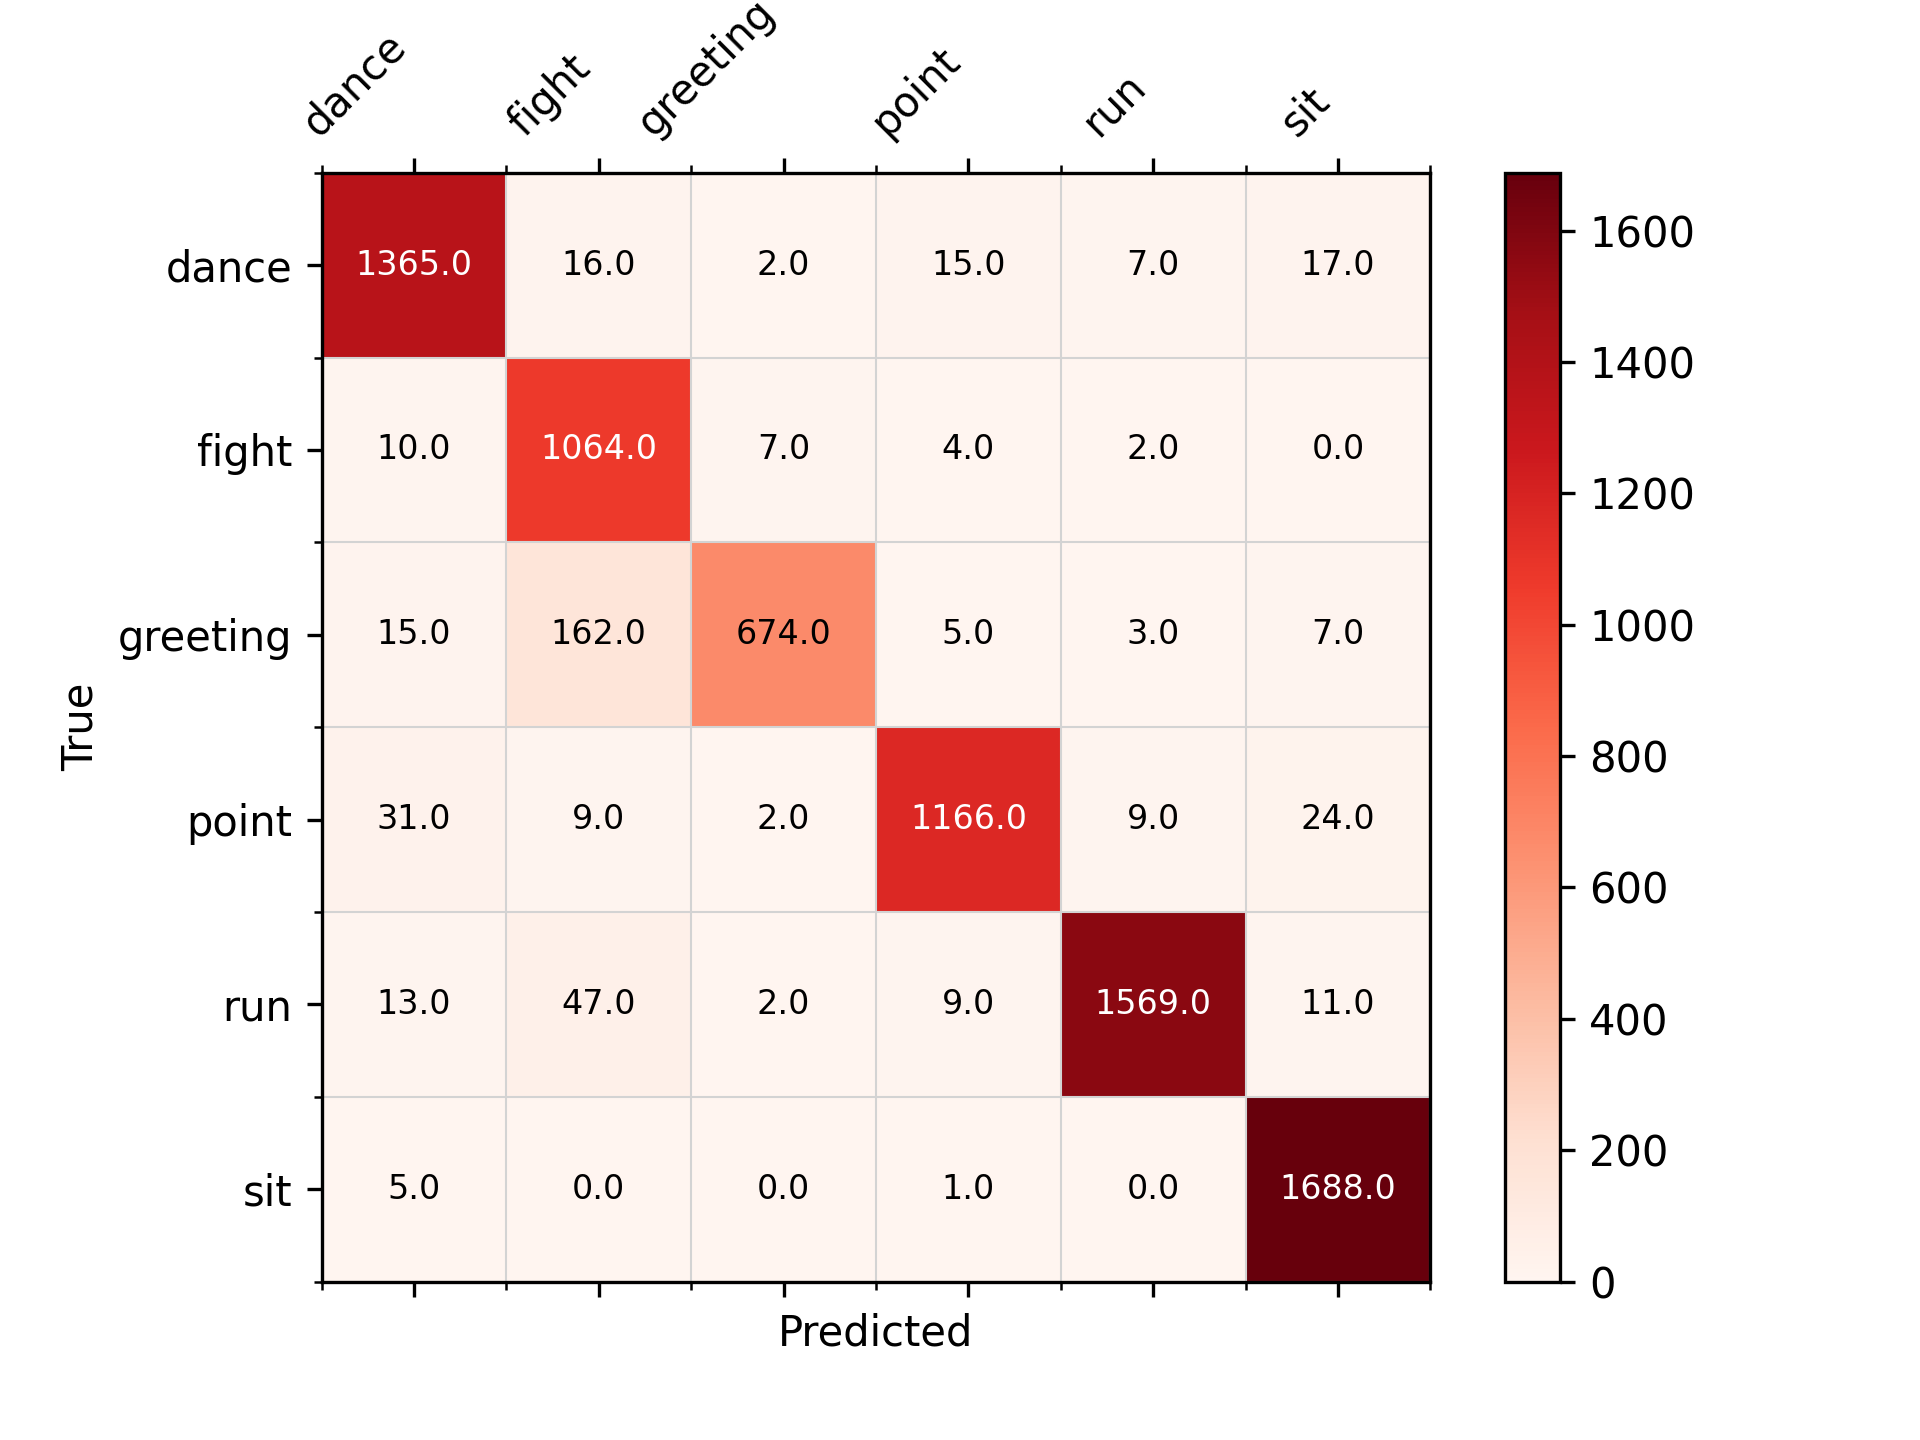
\includegraphics[width=0.6\textwidth]{Imagenes/Bitmap/CM_best_rf_0.2.png}
    \caption{Matriz de confusión del modelo Random Forest con 0.2s de intervalo (mejor val\_accuracy = 0.85735)}
    \label{fig:rf-0.2-matriz}
\end{figure}

\section{Intervalo 0.4s}

\begin{figure}[H]
    \centering
    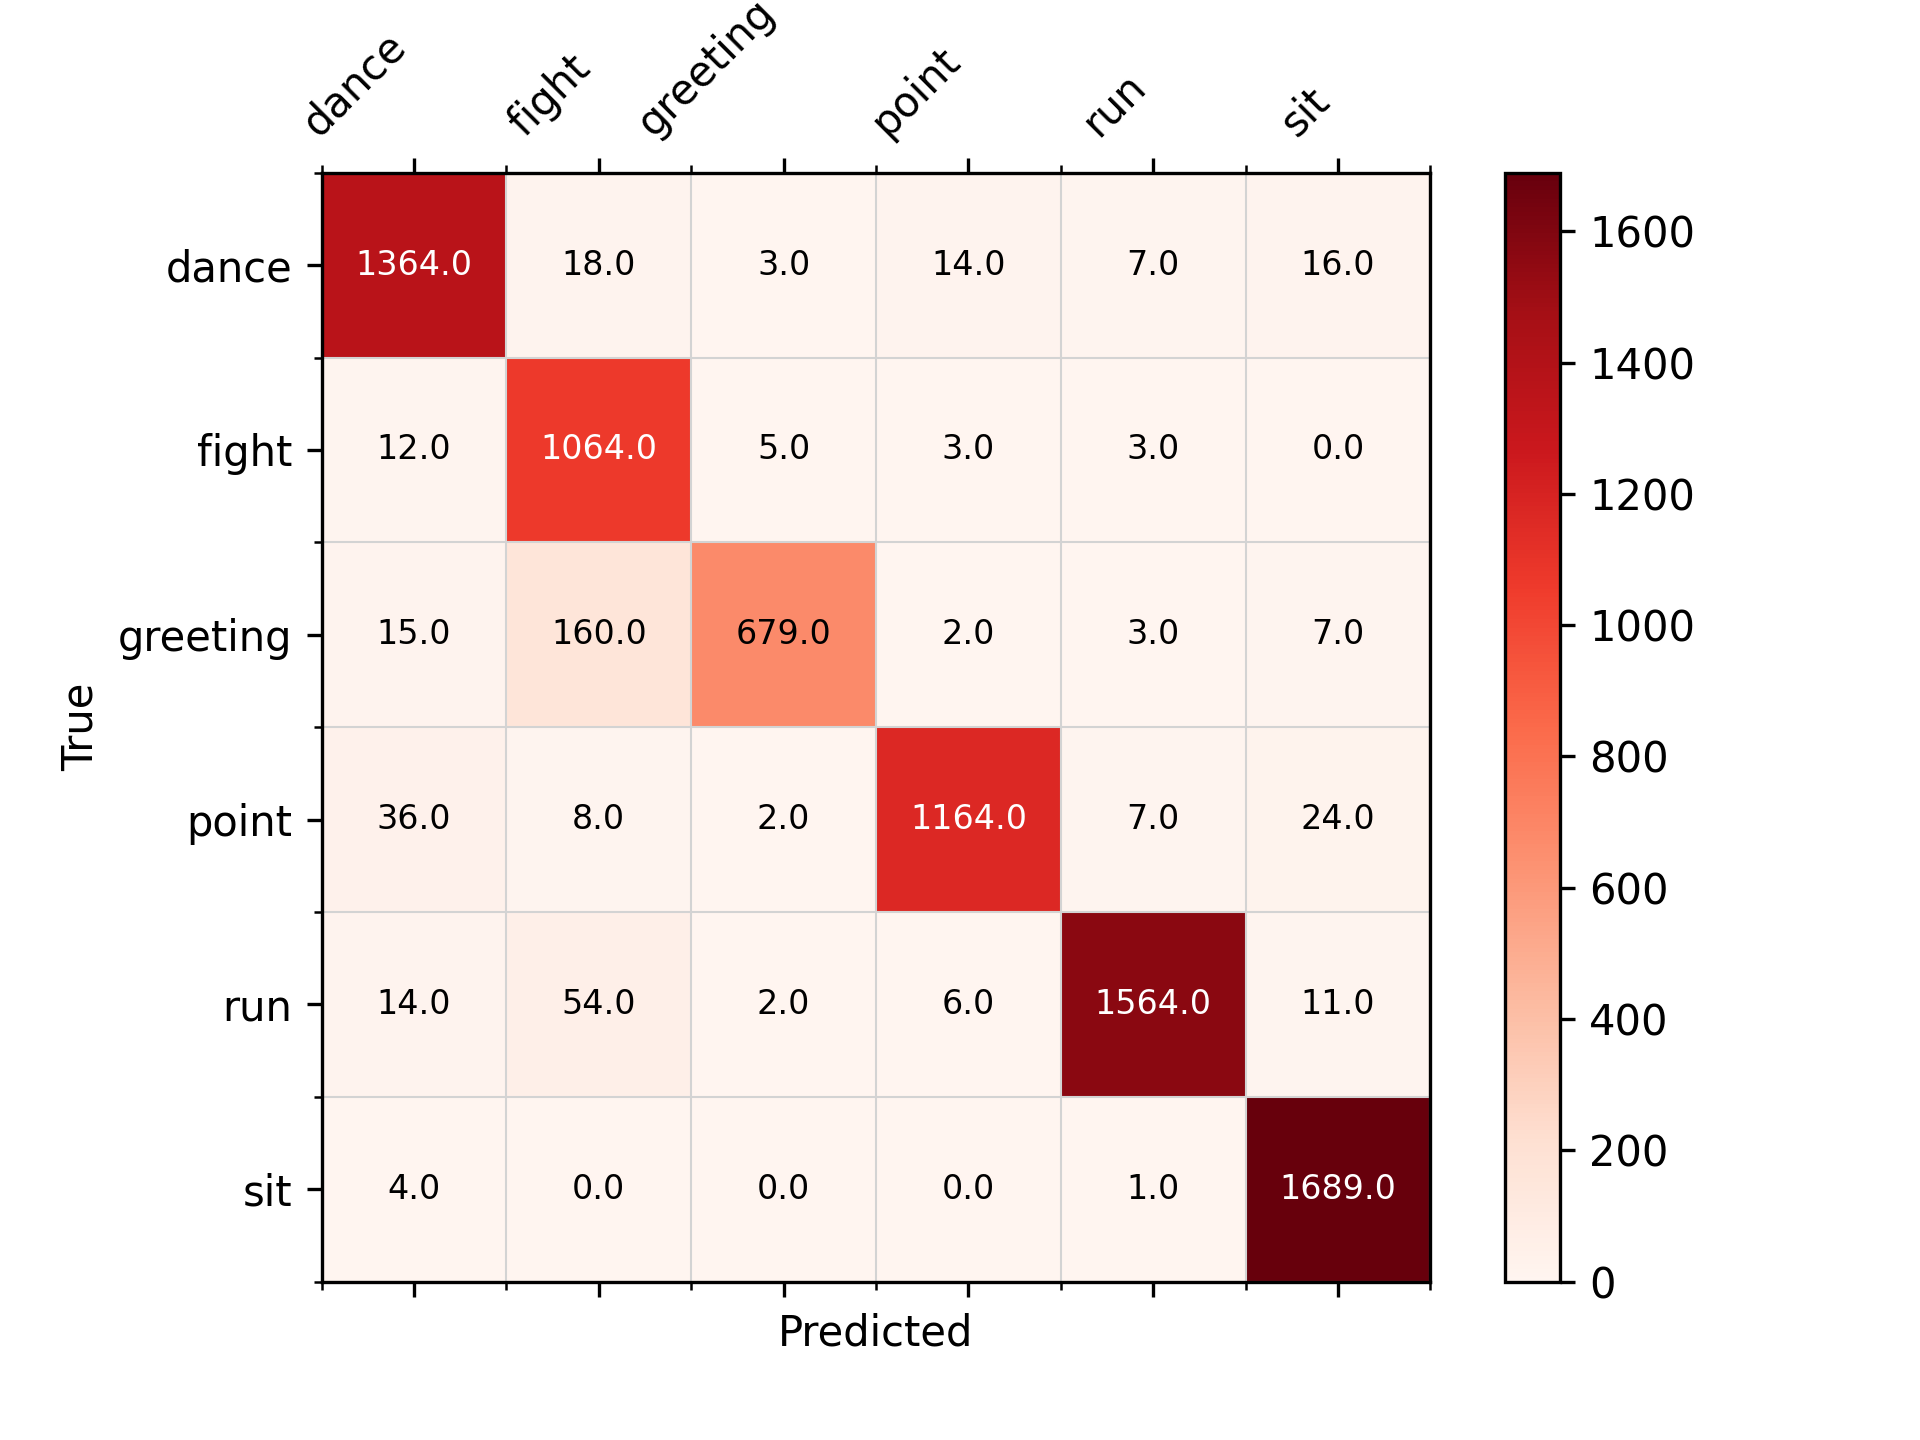
\includegraphics[width=0.6\textwidth]{Imagenes/Bitmap/CM_best_rf_0.4.png}
    \caption{Matriz de confusión del modelo Random Forest con 0.4s de intervalo (mejor val\_accuracy = 0.85735)}
    \label{fig:rf-0.4-matriz}
\end{figure}

\section{Intervalo 0.6s}

\begin{figure}[H]
    \centering
    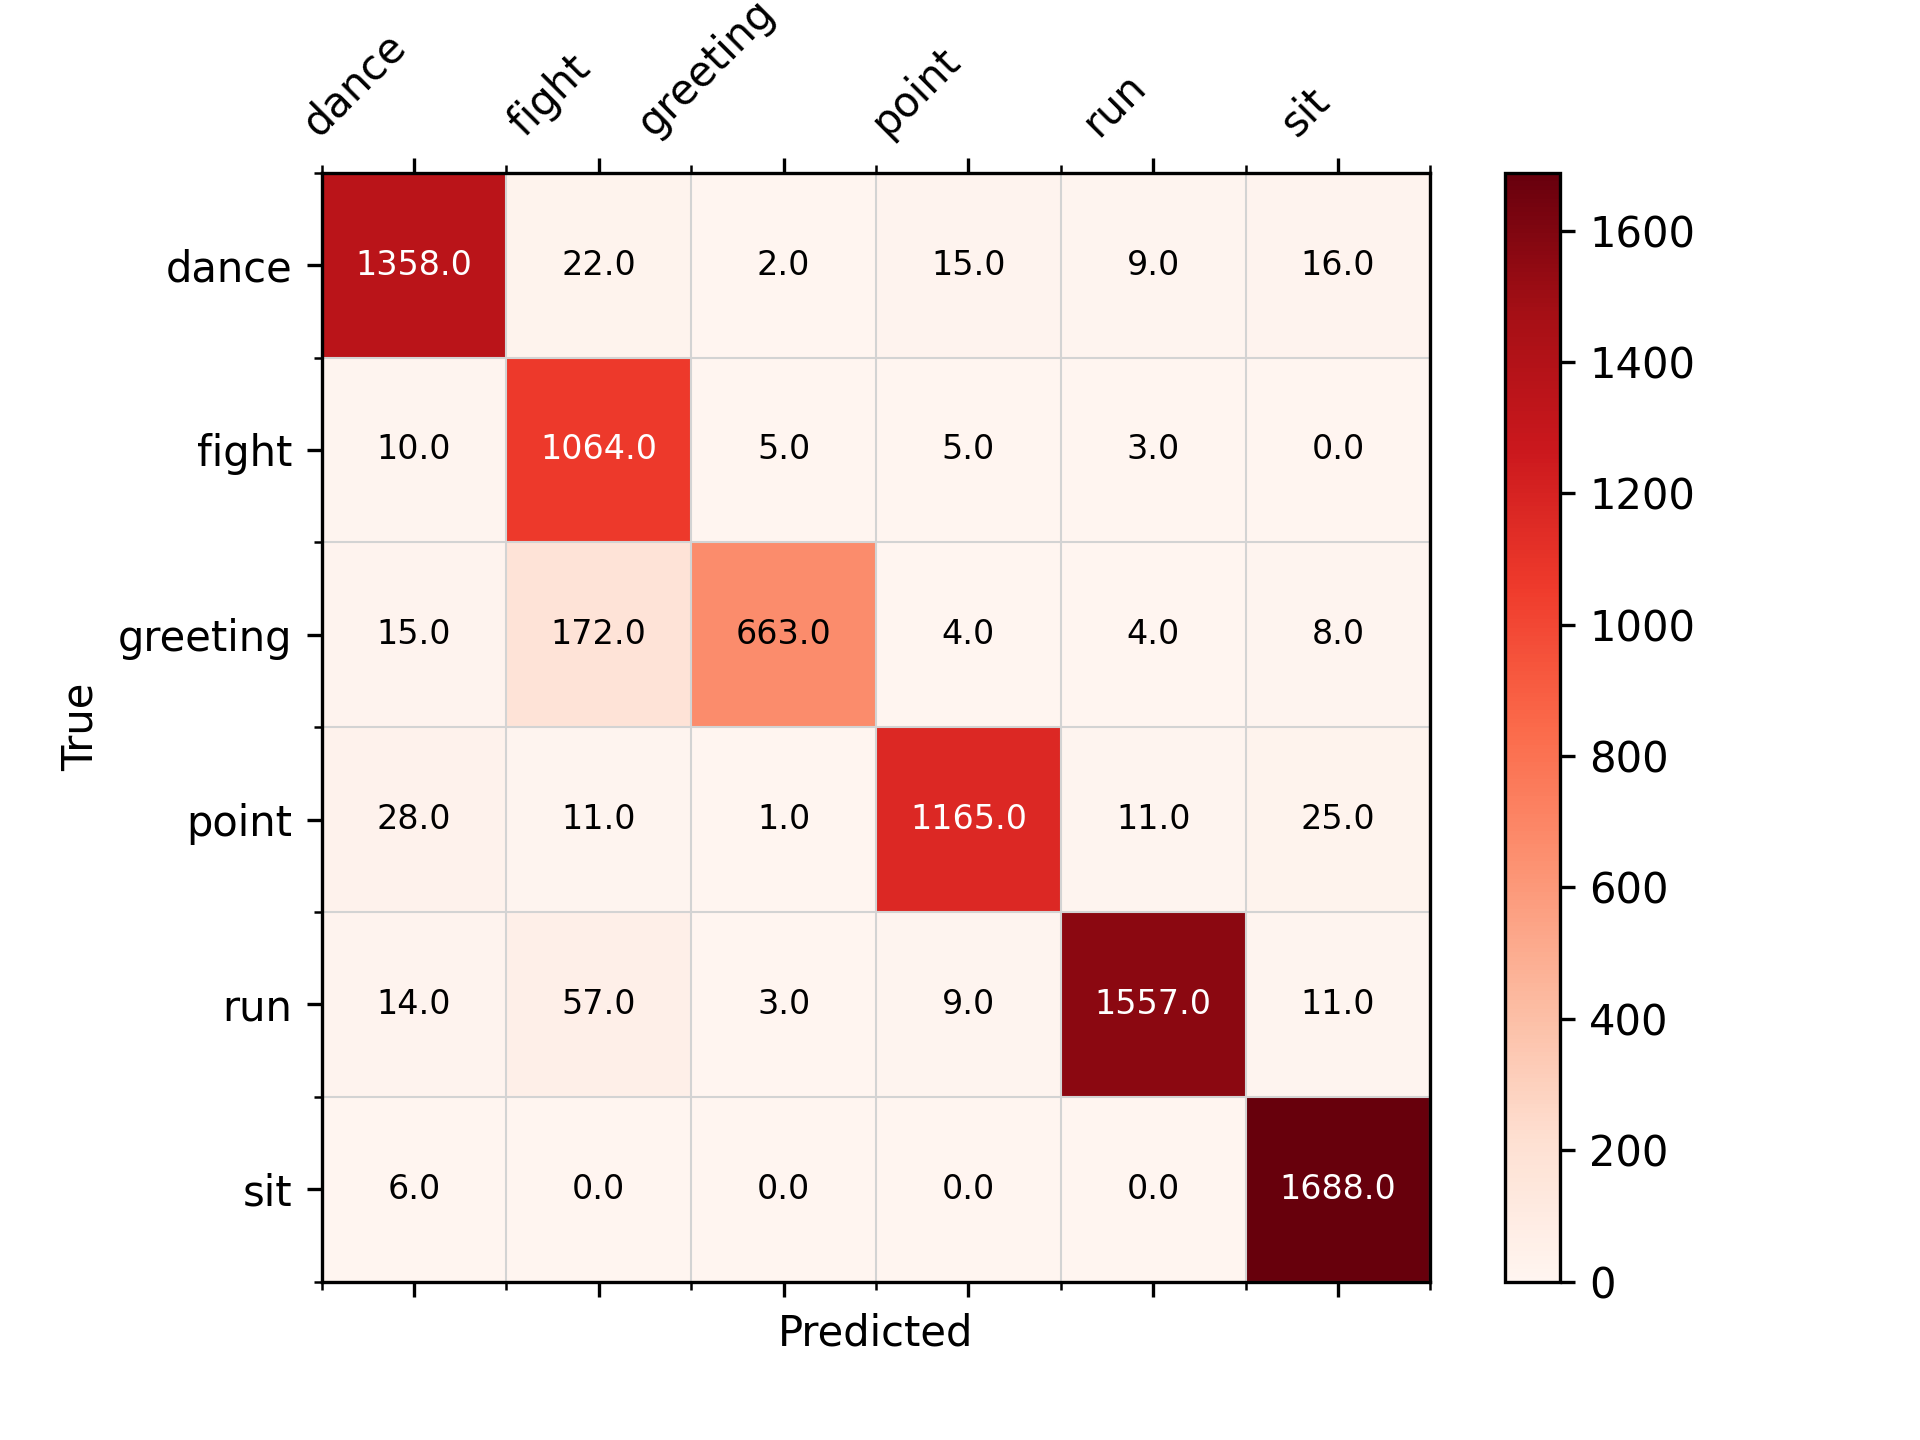
\includegraphics[width=0.6\textwidth]{Imagenes/Bitmap/CM_best_rf_0.6.png}
    \caption{Matriz de confusión del modelo Random Forest con 0.6s de intervalo (mejor val\_accuracy = 0.85233)}
    \label{fig:rf-0.6-matriz}
\end{figure}

\section{Intervalo 0.8s}

\begin{figure}[H]
    \centering
    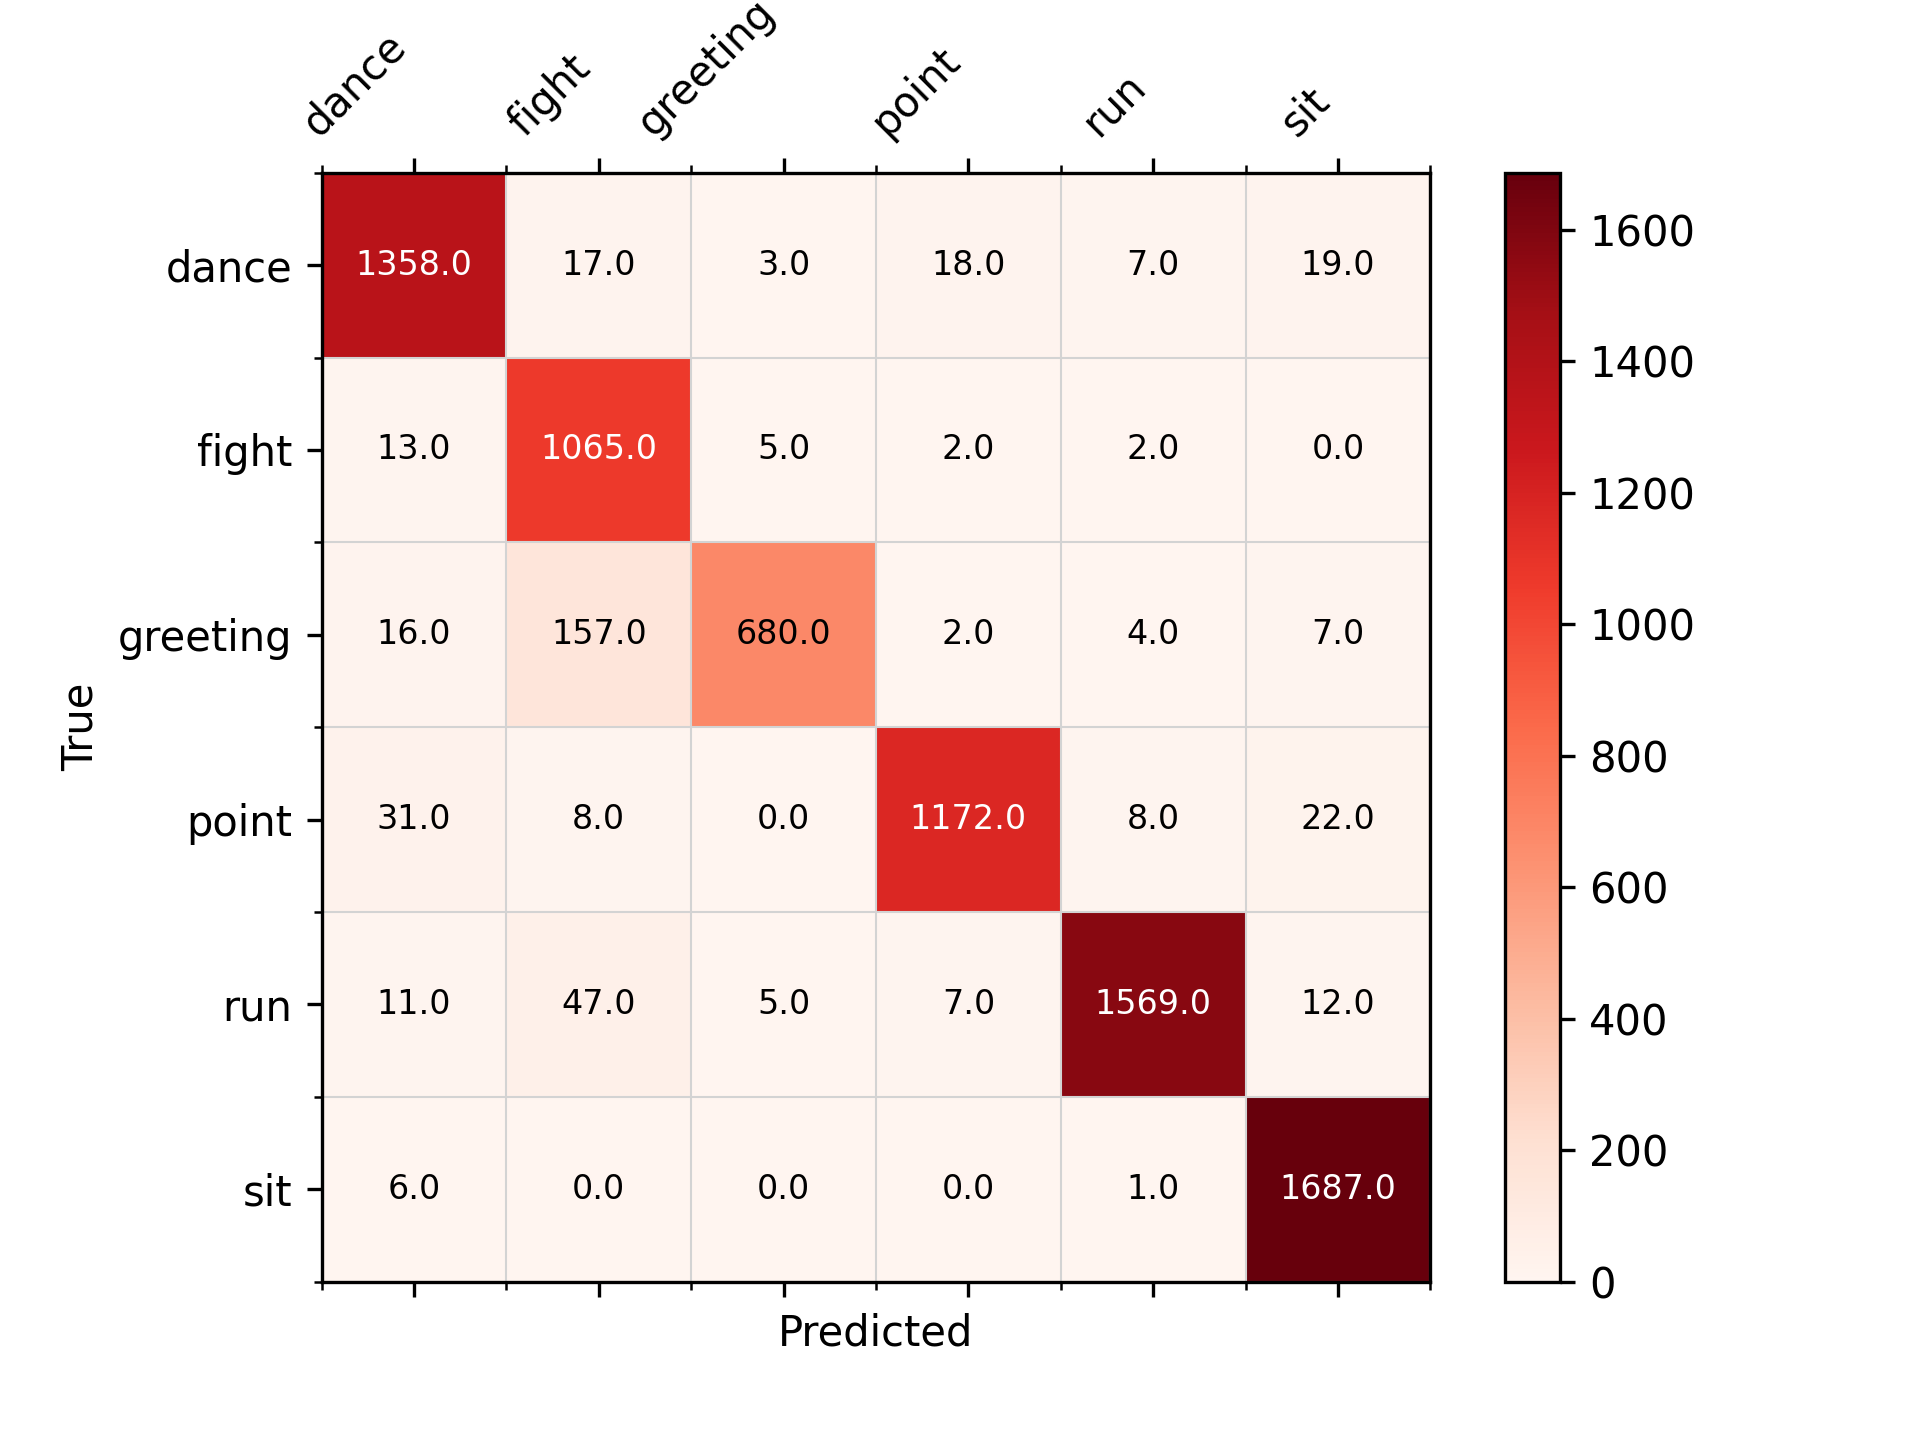
\includegraphics[width=0.6\textwidth]{Imagenes/Bitmap/CM_best_rf_0.8.png}
    \caption{Matriz de confusión del modelo Random Forest con 0.8s de intervalo (mejor val\_accuracy = 0.85936)}
    \label{fig:rf-0.8-matriz}
\end{figure}

\section{Intervalo 1.0s}

\begin{figure}[H]
    \centering
    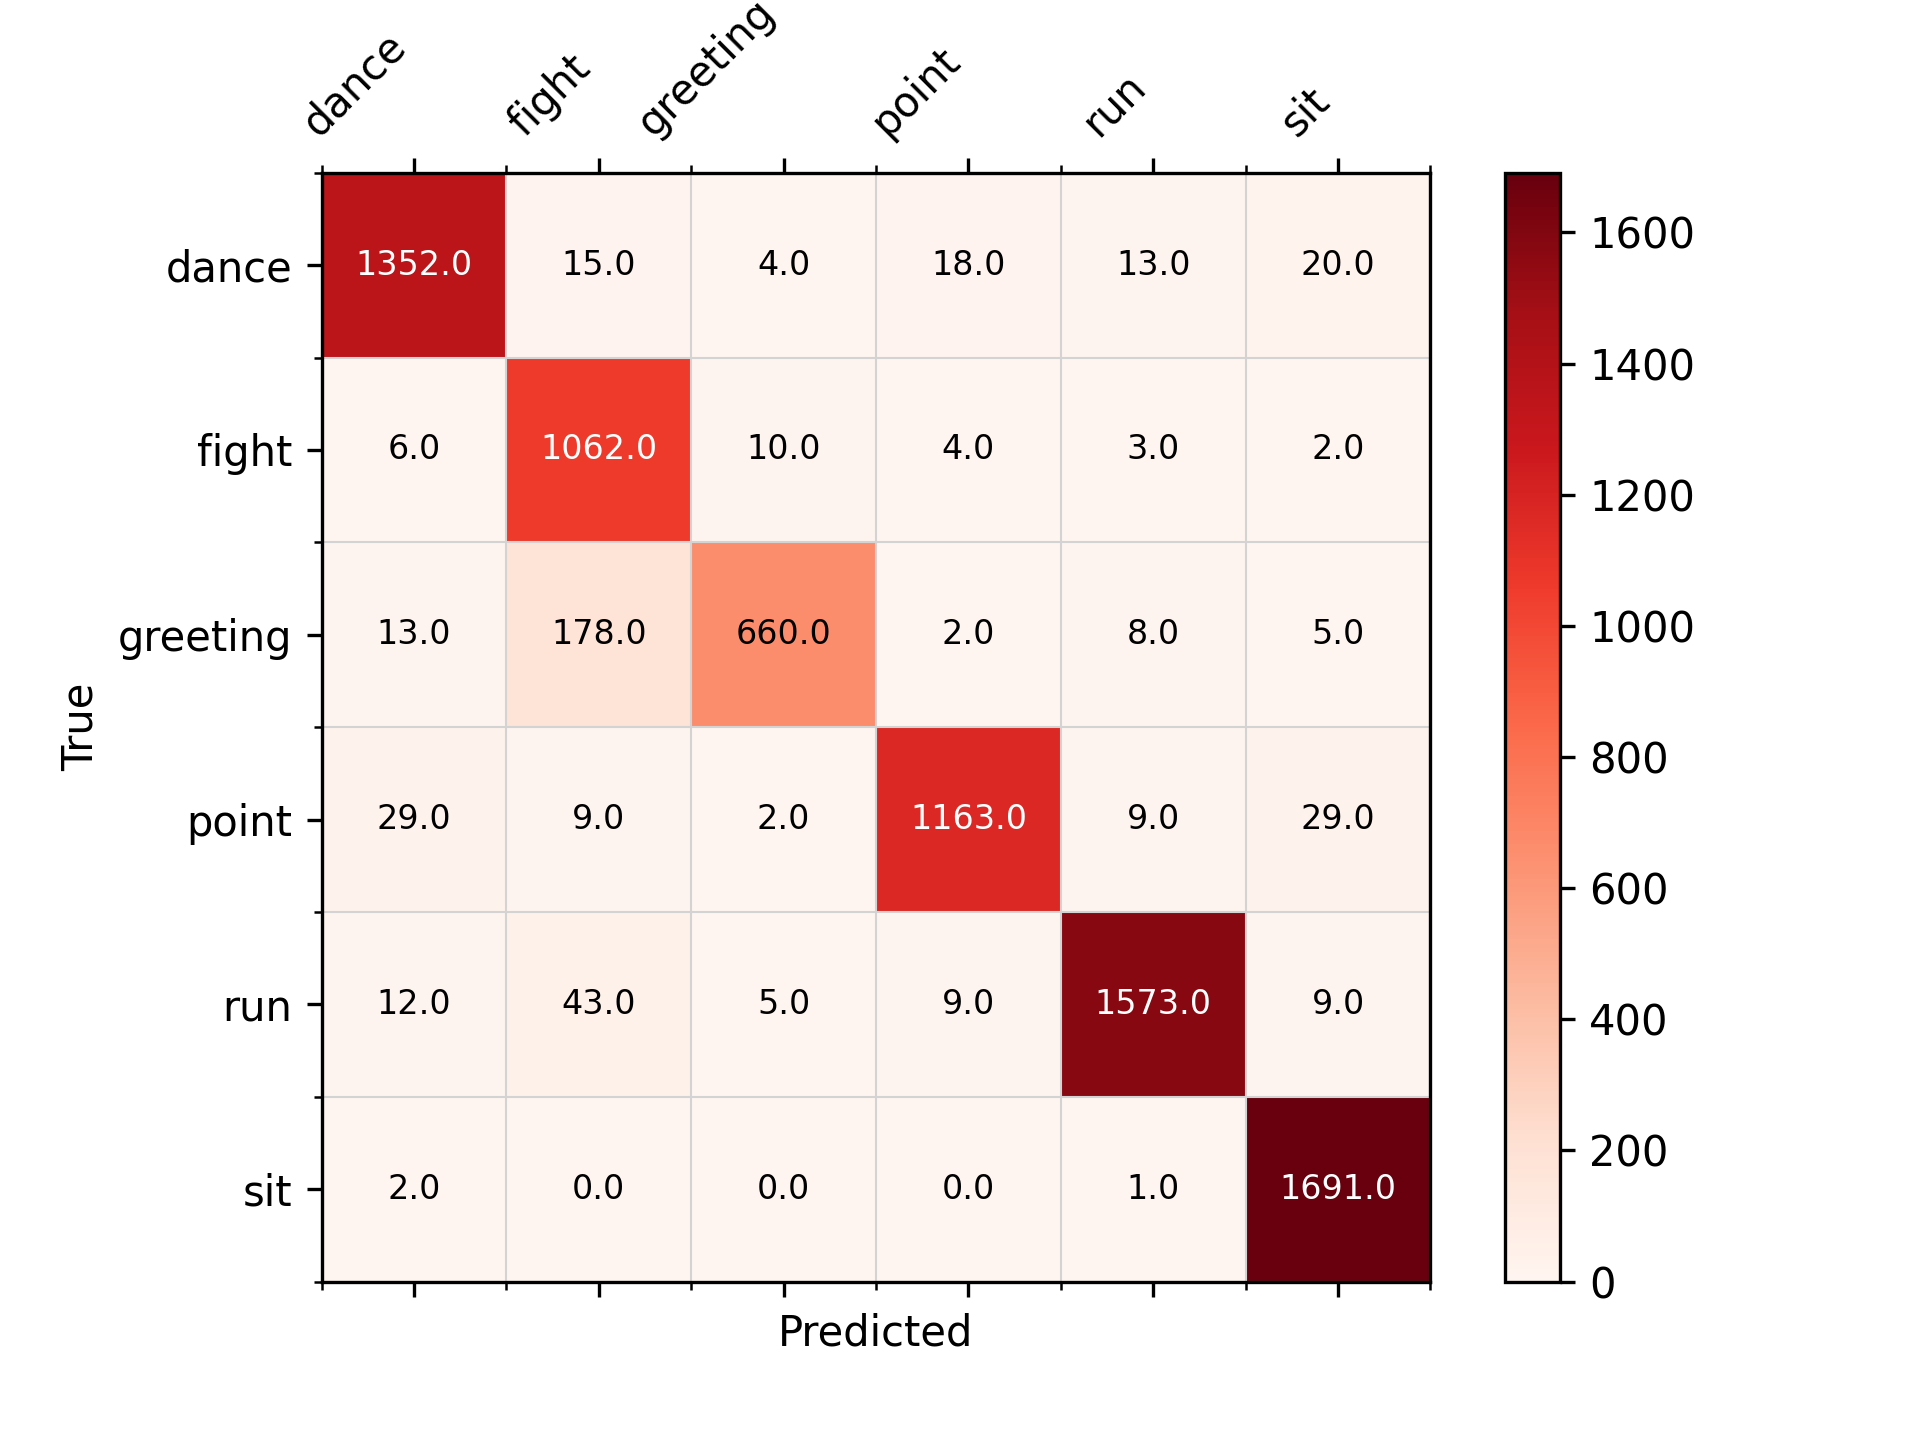
\includegraphics[width=0.6\textwidth]{Imagenes/Bitmap/CM_best_rf_1.0.png}
    \caption{Matriz de confusión del modelo Random Forest con 1.0s de intervalo (mejor val\_accuracy = 0.84681)}
    \label{fig:rf-1.0-matriz}
\end{figure}